\documentclass[twocolumn]{extarticle}
\usepackage{fontspec}   %加這個就可以設定字體
\usepackage{xeCJK}       %讓中英文字體分開設置
\usepackage{indentfirst}
\usepackage{listings}
\usepackage[newfloat]{minted}
\usepackage{float}
\usepackage{graphicx}
\usepackage{caption}
\usepackage{fancyhdr}
\usepackage{hyperref}
\usepackage{amsmath}
\usepackage{multirow}
\usepackage[dvipsnames]{xcolor}
\usepackage{graphicx}
\usepackage{tabularx}
\usepackage{booktabs}
\usepackage{caption}
\usepackage{subcaption}
\usepackage{pifont}
\usepackage{amssymb}
\usepackage{titling}

\usepackage{pdftexcmds}
\usepackage{catchfile}
\usepackage{ifluatex}
\usepackage{ifplatform}

\usepackage[breakable, listings, skins, minted]{tcolorbox}
\usepackage{etoolbox}
\setminted{fontsize=\footnotesize}
\renewtcblisting{minted}{%
    listing engine=minted,
    minted language=verilog,
    listing only,
    breakable,
    enhanced,
    minted options = {
        linenos, 
        breaklines=true, 
        breakbefore=., 
        % fontsize=\footnotesize, 
        numbersep=2mm
    },
    overlay={%
        \begin{tcbclipinterior}
            \fill[gray!25] (frame.south west) rectangle ([xshift=4mm]frame.north west);
        \end{tcbclipinterior}
    }   
}

\usepackage[
top=1.5cm,
bottom=0.75cm,
left=1.5cm,
right=1.5cm,
includehead,includefoot,
heightrounded, % to avoid spurious underfull messages
]{geometry} 

\newenvironment{code}{\captionsetup{type=listing}}{}
\SetupFloatingEnvironment{listing}{name=Code}
\usepackage[moderate]{savetrees}


\title{Introduction to Image Processing HW4}
\author{110550088 李杰穎}
\date{\today}


\setCJKmainfont{Noto Serif TC}


\ifwindows
\setmonofont[Mapping=tex-text]{Consolas}
\fi

\XeTeXlinebreaklocale "zh"             %這兩行一定要加,中文才能自動換行
\XeTeXlinebreakskip = 0pt plus 1pt     %這兩行一定要加,中文才能自動換行

\setlength{\parindent}{0em}
\setlength{\parskip}{1em}
\renewcommand{\baselinestretch}{1.25}
\setlength{\droptitle}{-7.5em}   % This is your set screw
\setlength{\columnsep}{2em}

\begin{document}

\maketitle

\section{Method}

In this homework, I first used Fourier transform and observe the spectrum of provided two images. After observing the spectrum, I designed the corresponding masks that filtered out the noises. It's worth noting that after generating patterns in masks, I used a Gaussian filter to make masks smoother. This will avoid alias problem that ideal filter 
would meet.

\subsection{Implementation Detail}

I directly used \texttt{np.fft.fft2} function for discrete Fourier Transform, the 2 in the function name means 2 dimensions. In order to make spectrum clearer, I also used \texttt{np.fft.fftshift} to shift the zero-frequency component to the center of the spectrum.

For generating masks, I first used \texttt{np.ones((h, w), np.uint8) * 255.0} to initialize the mask array, and used \texttt{cv2.line} and \texttt{cv2.circle} to draw circles and lines fill with 0 on mask. After drawing lines and circles, I used Gaussian Blur(\texttt{cv2.GaussianBlur}) to blur the masks.

\subsection{Image 1}

As we can observe in \autoref{fig:result}, the spectrum of image 1 has vertical lines across the whole spectrum. As mentioned in class, the vertical lines in the spectrum indicates the horizontal stripe appears in the original image 1. To remove the noise, we can used ``vertical notch reject filter'' which is a vertical lines with middle part leave opened. The reason why we need to leave the middle part opened is because we removes the zero-frequency term, the corresponding images will have its average pixel values equals to 0, which is not ideal.

The width of line is 5 pixels, and the width of open middle part is 25 pixels. And the kernel size of Gaussian blur is 21.

After applying Gaussian blur, just multiply the mask with the spectrum, and then apply inverse shifting, invert Fourier transform and \texttt{abs()} to get filtered image

\subsection{Image 2}

As we can observe in \autoref{fig:result}, the spectrum of image 2 has 12 white crosses. I used circle with radius equals to 15 pixels to filter out the crosses. After generating circles, I used Gaussian blur with kernel size equals to 31 to blur the whole masks.

The process after applying Gaussian blur is identical as in image 1.

\section{Result}

As we can see in \autoref{fig:result}, the noises in right-most images are significantly decreased. The images become clearer.

\begin{figure*}[b]
\centering
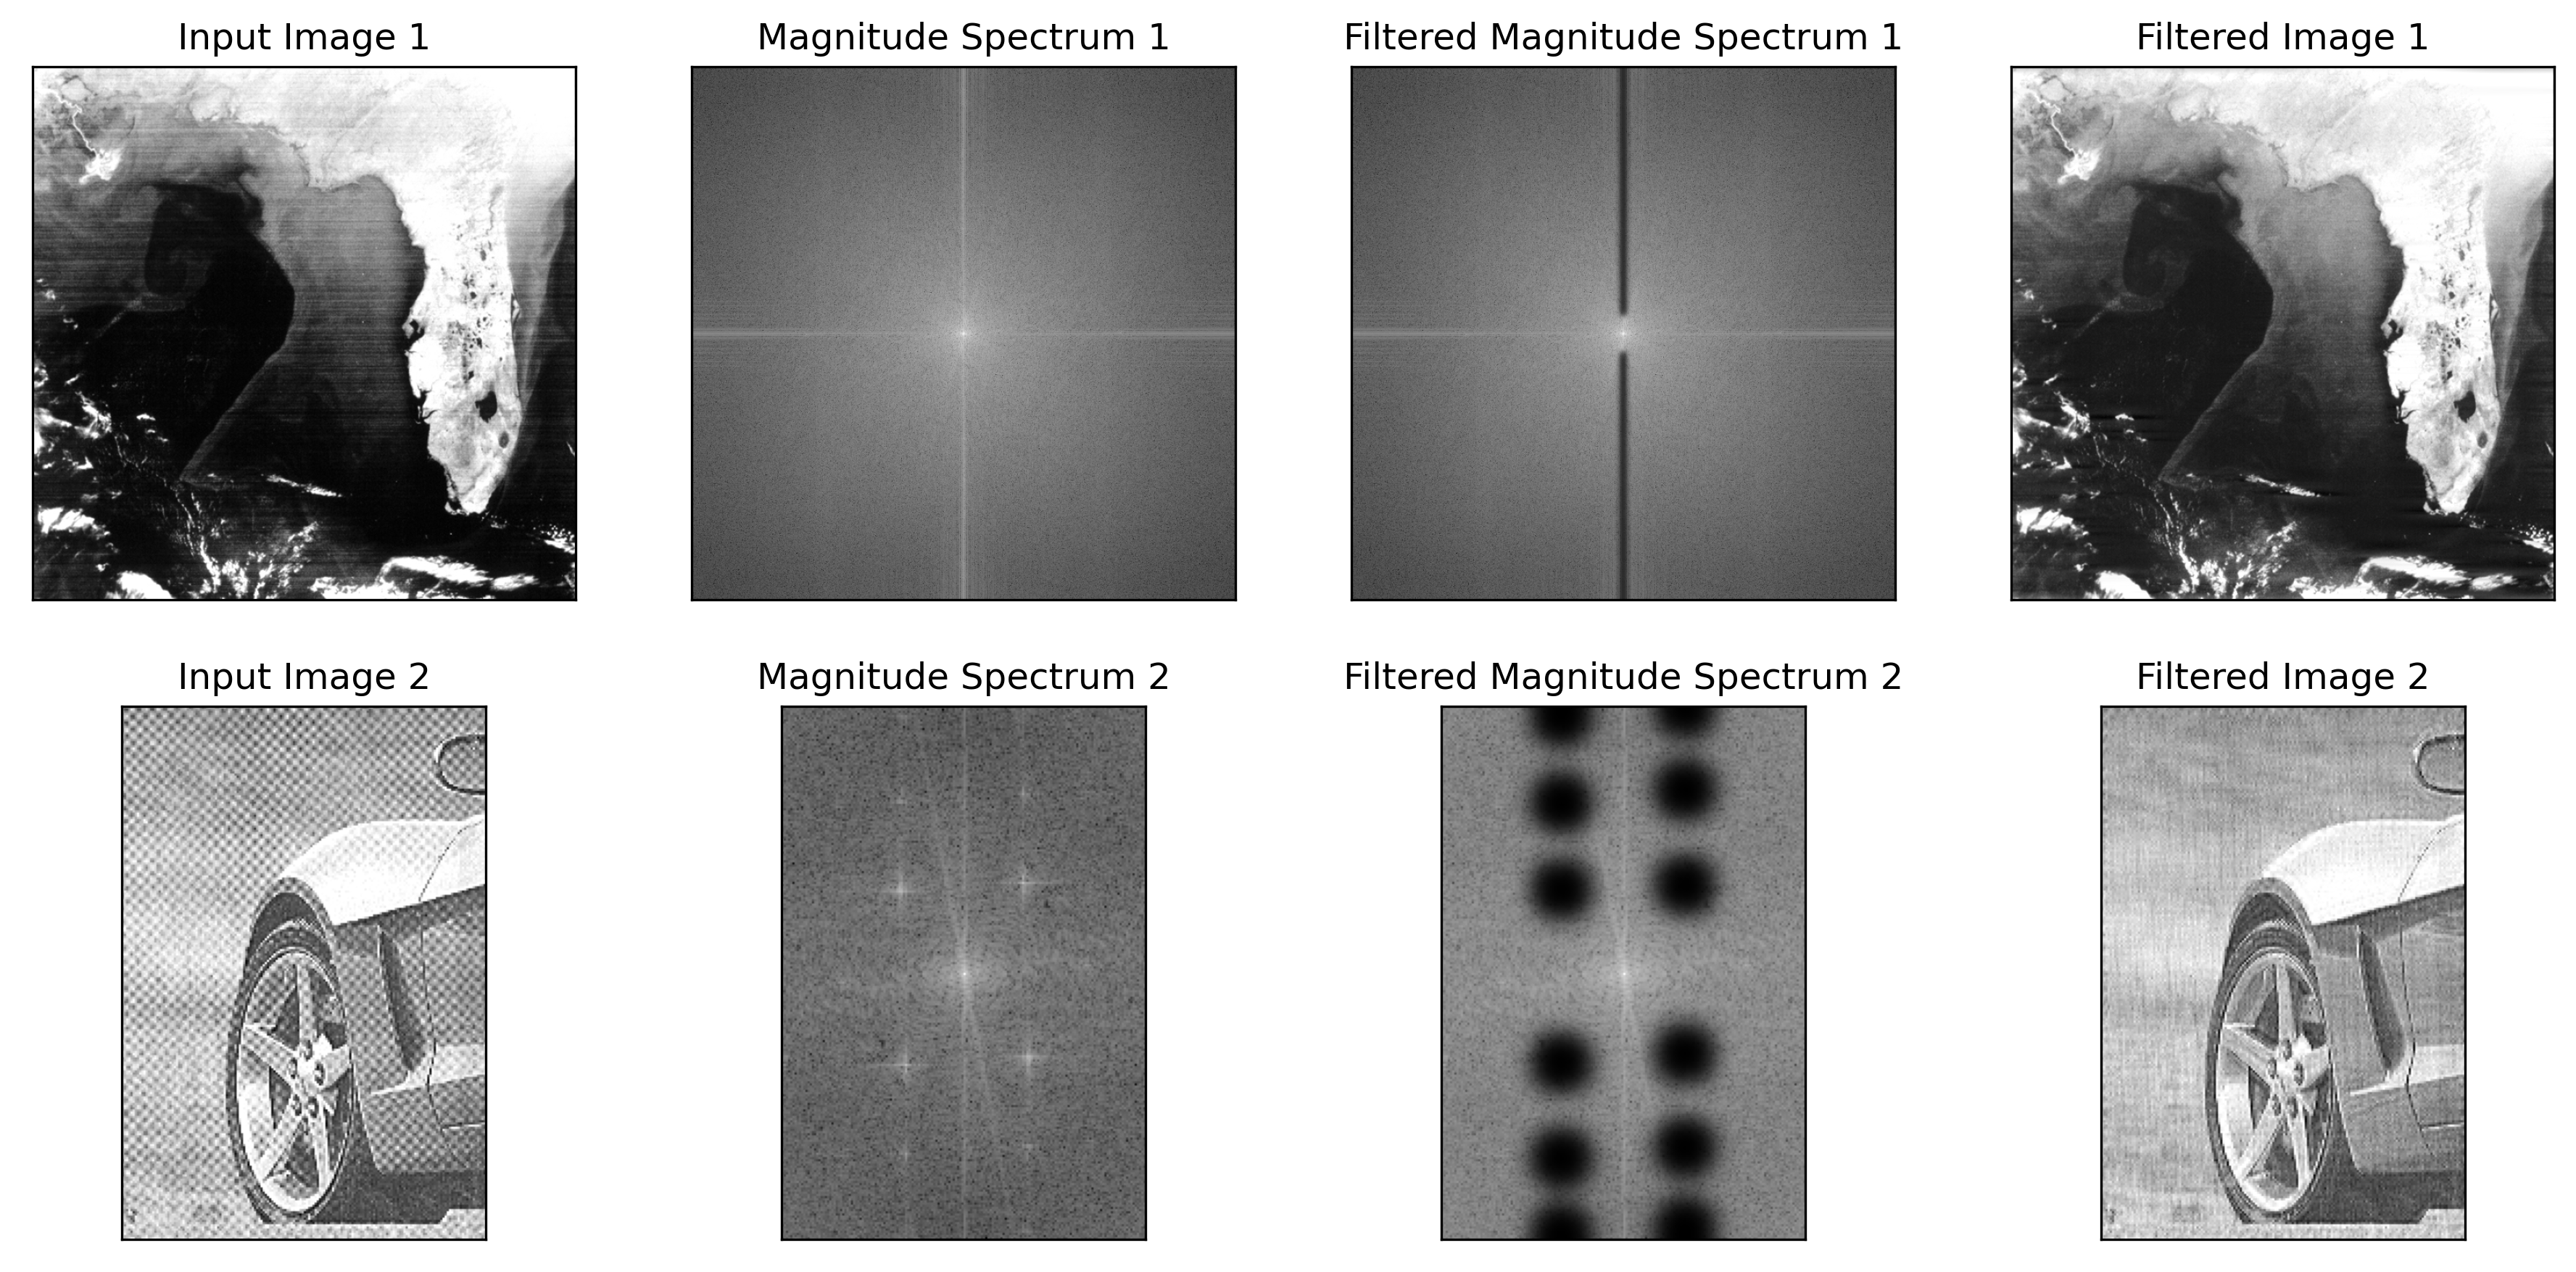
\includegraphics[width=0.95\linewidth]{result}
\caption{The final results of this homework, the right-most images are images after denoising.}
\label{fig:result}
\end{figure*}


\section{Feedback}

In this homework, I learned how to used \texttt{cv2} and \texttt{numpy} to apply Fourier transform to grayscale images, also learned how to design masks by observing the spectrum, and used the masks to filter out the noises in original images.


\end{document}